% Fase 5: exemplos clinicos do capitulo 6 (11, 12, 13, 14, 18)
% e comparacoes externas reproduzidas do calibration/audit_report.html (MoeaBench v0.14.0).
% Nao misturar protocolos: monografia e relatorio sao estudos distintos.
\setlength{\parskip}{4pt}

\begin{frame}[plain]
\vspace*{2cm}
{\LARGE\color{navy}Exemplos clínicos e comparações\par}
\vspace{.24cm}
{\large Diagnósticos FAIR aplicados a DTLZ e DPF\par}
\vspace{.28cm}
\textcolor{navy!40}{\rule{.75\linewidth}{.6pt}}\par
\vspace{.22cm}
Da métrica física ao Q-score e à interpretação geométrica.
\end{frame}

\begin{frame}[fragile]{Exemplo FAIR 11 — Um diagnóstico em dois problemas DPF}
\textbf{Pergunta:} quantas soluções não dominadas encontramos e quão bem elas representam a referência do problema?
\begin{columns}[T,onlytextwidth]
\begin{column}{.53\textwidth}
\begin{lstlisting}[style=python,basicstyle=\ttfamily\fontsize{7.6}{9.5}\selectfont]
exp1.mop = mb.mops.DPF1(M=3)
exp1.moea = mb.moeas.NSGA3(population=92)
exp1.run(generations=150)
mb.clinic.audit(exp1).report()

exp2.mop = mb.mops.DPF2(M=3)
exp2.moea = mb.moeas.MOEAD(population=92)
exp2.run(generations=150)
mb.clinic.audit(exp2).report()
\end{lstlisting}
\end{column}
\begin{column}{.45\textwidth}
\textbf{DPF1 / NSGA-III:} 18 não dominadas; 74 dominadas. A auditoria aponta proximidade favorável, mas deficiências de cobertura e organização espacial.
\par\medskip
\textbf{DPF2 / MOEA/D:} 90 não dominadas; 2 dominadas. Apesar disso, observa-se afastamento importante da referência.
\end{column}
\end{columns}
\vspace{.08cm}
\textbf{Interpretação:} não dominância é relativa às soluções encontradas; ela não prova proximidade à frente ótima nem boa distribuição.
\end{frame}

\begin{frame}{Exemplo FAIR 11 — As geometrias explicam o contraste}
\begin{columns}[T,onlytextwidth]
\begin{column}{.49\textwidth}\centering
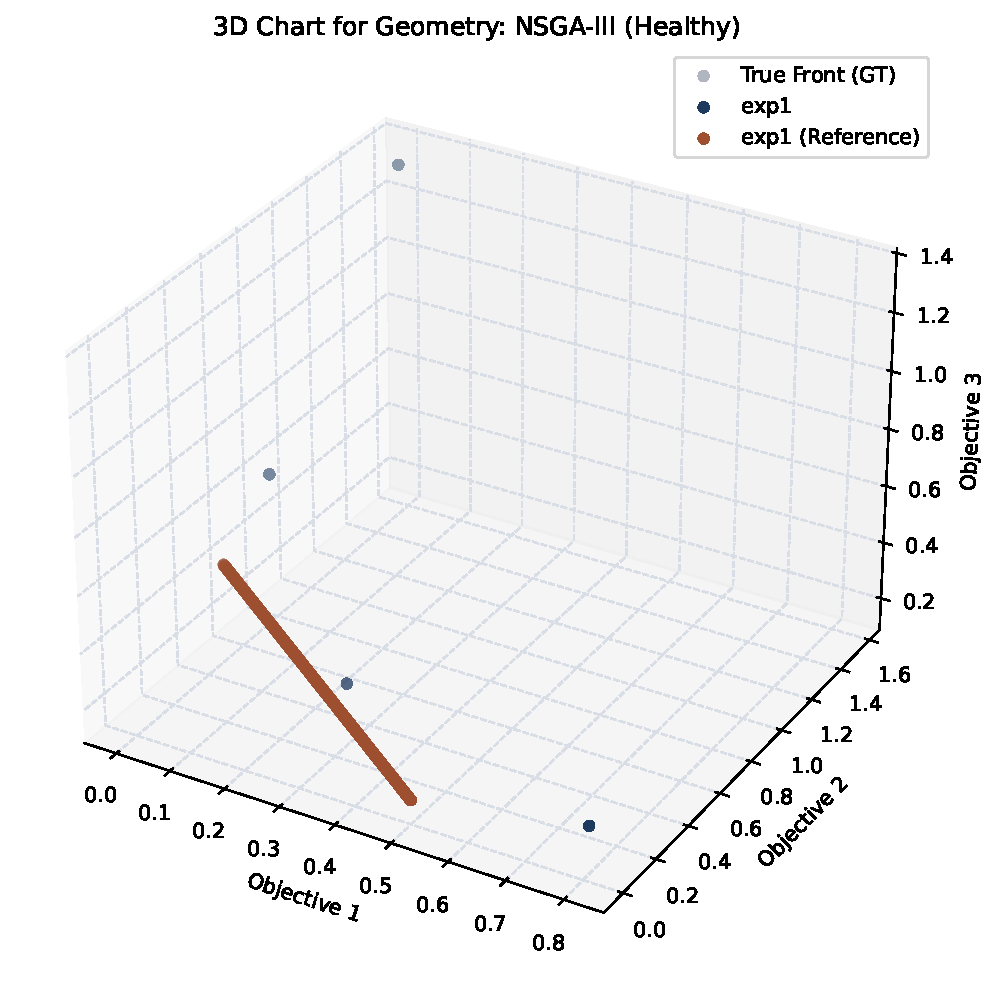
\includegraphics[width=\linewidth,height=.51\textheight,keepaspectratio]{figures/example_11_01_topology.pdf}
\par\textbf{DPF1: NSGA-III}\par
\scriptsize 18 soluções não dominadas na população final.
\end{column}
\begin{column}{.49\textwidth}\centering
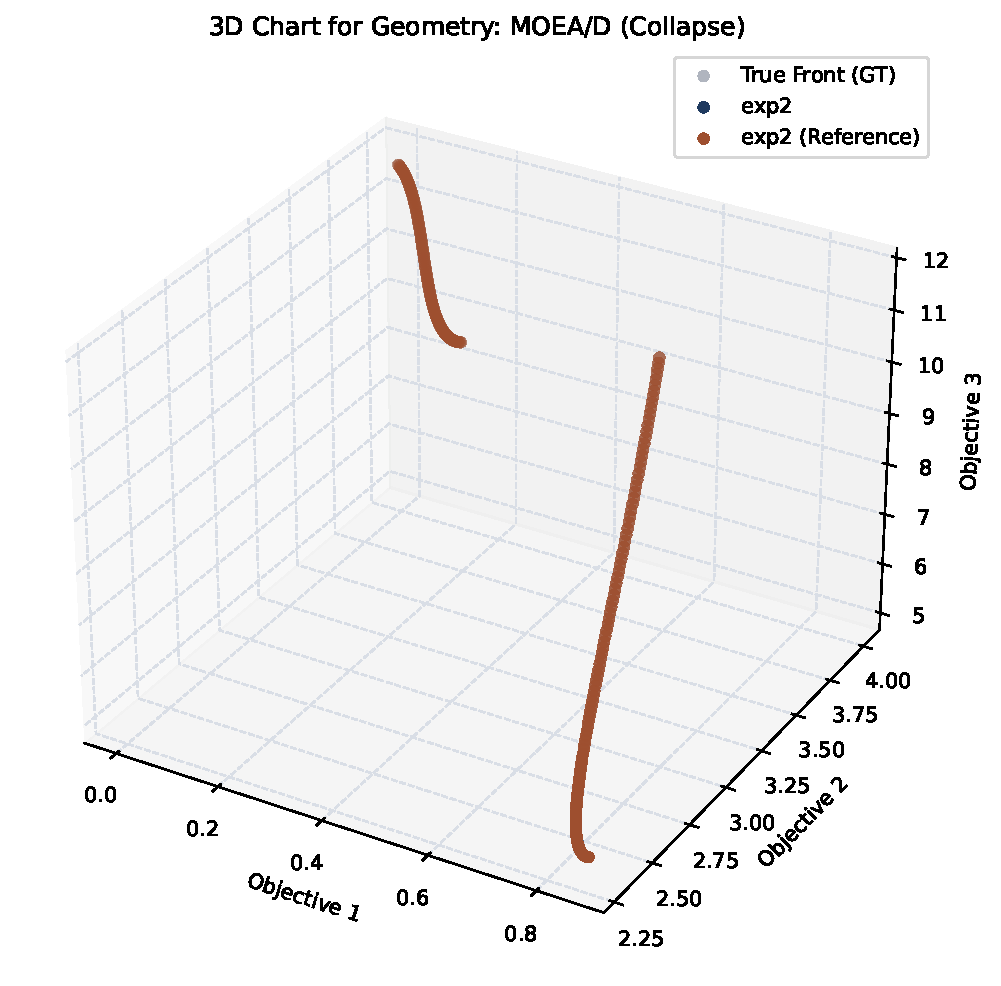
\includegraphics[width=\linewidth,height=.51\textheight,keepaspectratio]{figures/example_11_02_topology.pdf}
\par\textbf{DPF2: MOEA/D}\par
\scriptsize 90 soluções não dominadas na população final.
\end{column}
\end{columns}
\vspace{.09cm}
\textbf{Observe:} em DPF2, muitas soluções são mutuamente não dominadas, mas a nuvem está longe da referência. Os dois gráficos usam geometrias e GTs \emph{distintos}; não se trata de comparar distâncias absolutas entre DPF1 e DPF2.
\end{frame}

\begin{frame}[fragile]{Exemplo FAIR 12 — Medir os erros físicos antes de calibrar}
\textbf{DTLZ2, 3 objetivos; NSGA-II, 100 indivíduos, 30 gerações.} Referência analítica com 500 pontos.
\begin{columns}[T,onlytextwidth]
\begin{column}{.54\textwidth}
\begin{lstlisting}[style=python,basicstyle=\ttfamily\fontsize{7.5}{9.1}\selectfont]
gt = mop.pf(n_points=500)
exp1.run()
cl = mb.clinic.closeness(exp1, ref=gt)
cv = mb.clinic.coverage(exp1, ref=gt)
gp = mb.clinic.gap(exp1, ref=gt)
mb.clinic.audit(exp1, ground_truth=gt,
                quality=False).fr.report()
\end{lstlisting}
\textbf{Objetivo:} inspecionar as grandezas físicas diretamente, antes de convertê-las em Q-scores. Todas as seis medidas diferem em definição e interpretação.
\end{column}
\begin{column}{.43\textwidth}\centering
\renewcommand{\arraystretch}{1.20}
\begin{tabular}{@{}lr@{}}
\textbf{Métrica} & \textbf{Valor físico}\\\hline
Closeness & 0,0408\\
Coverage & 0,0859\\
Gap & 0,1527\\
Regularity & 0,0533\\
Balance & 0,2810\\
Headway & 0,1587\\
\end{tabular}
\end{column}
\end{columns}
\vspace{.11cm}
\textbf{Por exemplo:} o gap de 0,1527, baseado no percentil 95 das distâncias $R\to P$, evidencia uma cauda de regiões mais mal representadas do que a média de coverage (0,0859).
\end{frame}

\begin{frame}{Exemplo FAIR 12 — A medida deve ser lida na geometria}
\begin{columns}[T,onlytextwidth]
\begin{column}{.60\textwidth}\centering
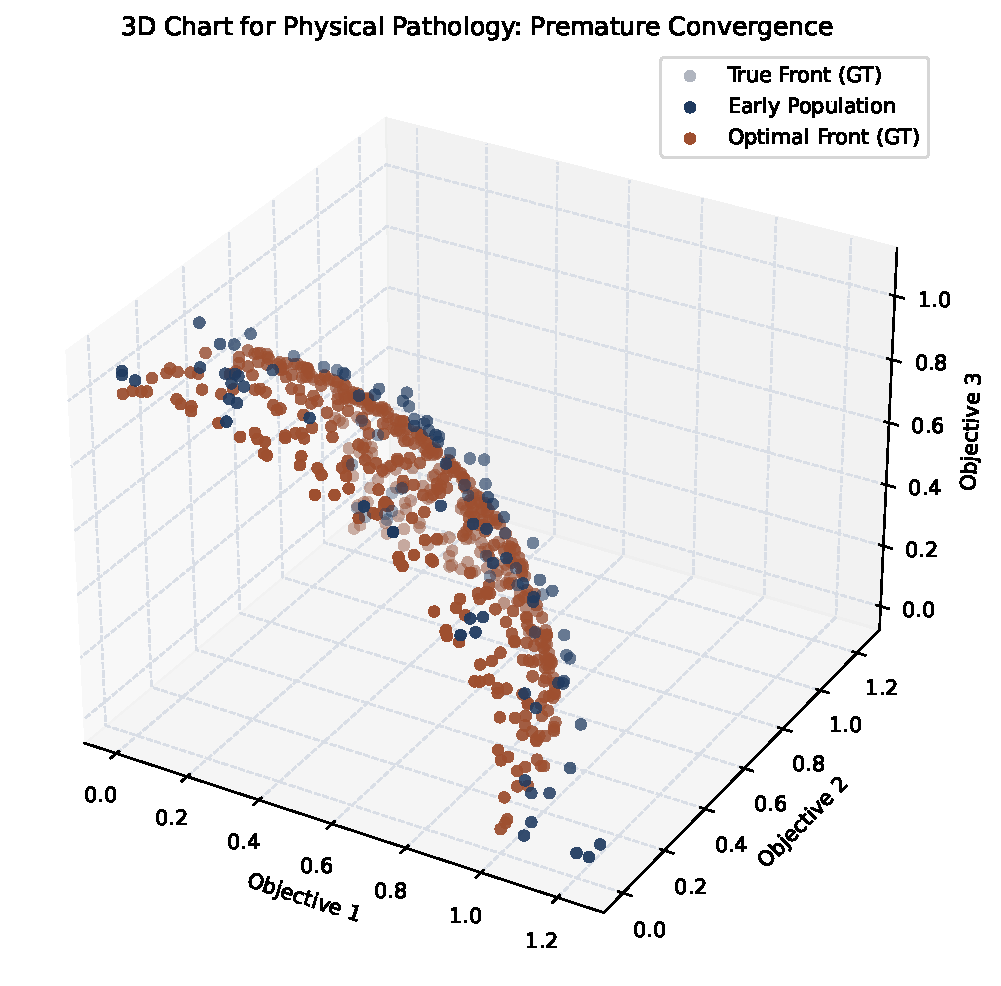
\includegraphics[width=\linewidth,height=.64\textheight,keepaspectratio]{figures/example_12_01_topology.pdf}
\par\scriptsize Pontos de referência, população inicial e população final.
\end{column}
\begin{column}{.38\textwidth}
\textbf{Closeness: 0,0408}\par\smallskip
As soluções finais estão próximas da superfície de referência.
\par\medskip
\textbf{Coverage: 0,0859}\par\smallskip
Parte da referência ainda se encontra a distâncias maiores da população.
\par\medskip
\textbf{Headway: 0,1587}\par\smallskip
O erro longitudinal final é cerca de 15,9\% do inicial: redução relativa de aproximadamente 84,1\%.
\end{column}
\end{columns}
\vspace{.05cm}\textbf{Limite da leitura:} esses números físicos não são porcentagens de ``qualidade''; só a calibração posterior produz escores comparáveis na régua 0--1.
\end{frame}

\begin{frame}[fragile]{Exemplo FAIR 13 — Q-scores revelam uma frente estruturalmente pobre}
\textbf{DTLZ1, 3 objetivos; NSGA-II, 100 indivíduos, 280 gerações; seed = 1.}
\begin{columns}[T,onlytextwidth]
\begin{column}{.52\textwidth}
\begin{lstlisting}[style=python,basicstyle=\ttfamily\fontsize{7.3}{9.3}\selectfont]
exp = mb.experiment()
exp.mop = mb.mops.DTLZ1(M=3)
exp.moea = mb.moeas.NSGA2(
    population=100, generations=280)
exp.run(seed=1)
gt = exp.optimal_front()
diag = mb.clinic.audit(exp,
    ground_truth=gt)
diag.quality.report(full=True)
mb.view.topology(exp, gt=gt,
                 markers=True)
\end{lstlisting}
\end{column}
\begin{column}{.46\textwidth}\centering
\renewcommand{\arraystretch}{1.12}
\begin{tabular}{@{}lr@{}}
\textbf{Q-score} & \textbf{Valor}\\\hline
Closeness & \textbf{0,883}\\
Coverage & 0,000\\
Gap & 0,000\\
Regularity & 0,000\\
Balance & 0,000\\
Headway & \textbf{0,999}\\
\end{tabular}
\end{column}
\end{columns}
\vspace{.10cm}\textbf{Leitura:} proximidade final e progresso foram favoráveis; cobertura, lacunas e distribuição receberam a pior classificação do protocolo. Um bom resultado em dois eixos não corrige quatro deficiências distintas.
\end{frame}

\begin{frame}{Exemplo FAIR 13 — Próximo da frente não implica cobrir a frente}
\begin{columns}[T,onlytextwidth]
\begin{column}{.61\textwidth}\centering
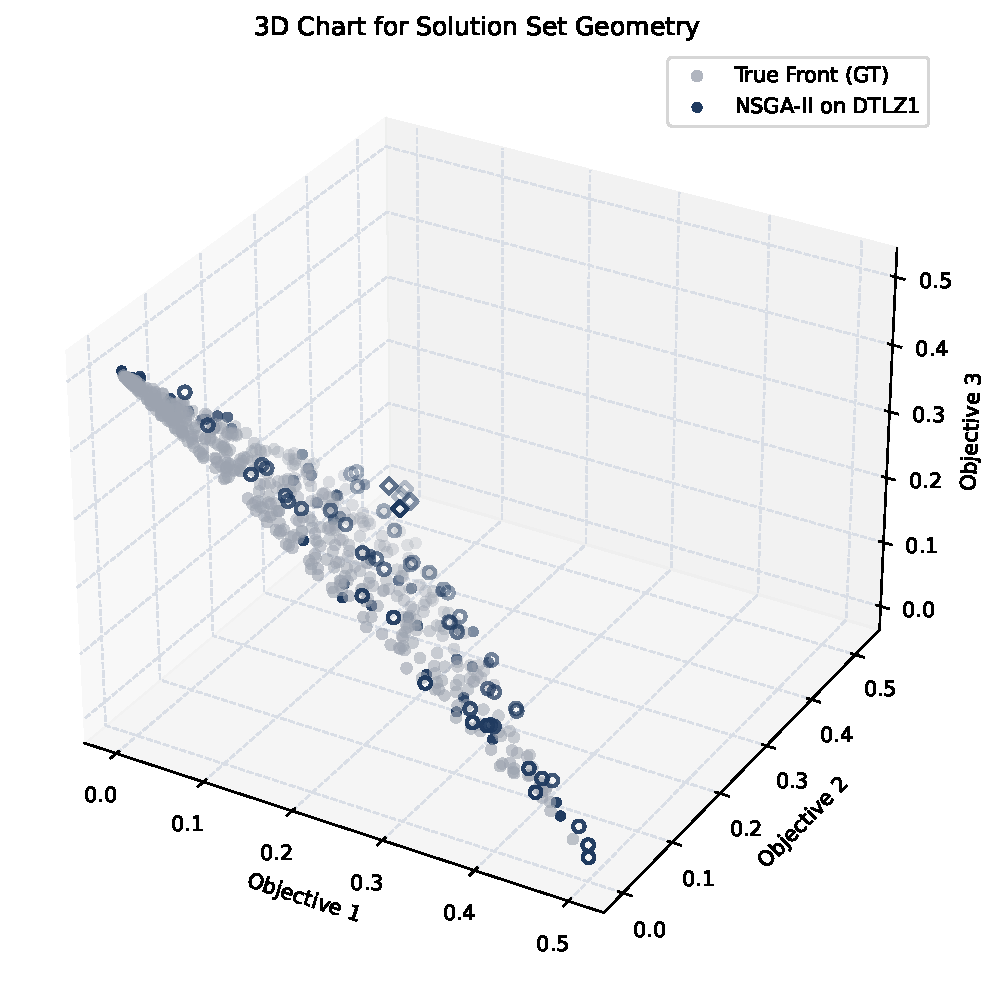
\includegraphics[width=\linewidth,height=.53\textheight,keepaspectratio]{figures/example_13_01_topology.pdf}
\par\scriptsize Referência DTLZ1 e soluções do NSGA-II na mesma geometria.
\end{column}
\begin{column}{.37\textwidth}
\textbf{O que observar?}\par\smallskip
As soluções aproximam-se da superfície de referência, mas permanecem agrupadas em porções limitadas.
\par\medskip
\textbf{Consequência}\par\smallskip
\emph{Closeness} e \emph{headway} altos coexistem com \emph{coverage}, \emph{gap}, \emph{regularity} e \emph{balance} nulos.
\end{column}
\end{columns}
\vspace{.03cm}\textbf{Conclusão:} o algoritmo encontrou parte da frente, mas deixou de representar adequadamente a diversidade dos compromissos. Essa deficiência não aparece em uma análise restrita à convergência.
\end{frame}

\begin{frame}[fragile]{Exemplo FAIR 14 — Do Q-score ao radar: perfil de DTLZ2}
\textbf{DTLZ2, 3 objetivos; NSGA-II, 100 indivíduos, 30 gerações.} Este é um experimento independente do exemplo 12.
\begin{columns}[T,onlytextwidth]
\begin{column}{.42\textwidth}
\begin{lstlisting}[style=python,basicstyle=\ttfamily\fontsize{7.4}{9}\selectfont]
gt = mop.pf(n_points=500)
exp1.run()
mb.view.radar(exp1,
    ground_truth=gt)
\end{lstlisting}
\textbf{Pergunta:} a aproximação foi boa em que dimensões e apresentou deficiência em quais outras?
\par\smallskip
\textbf{Interpretação:} closeness, coverage, gap e headway aparecem elevados; regularity é baixa e balance é intermediária-inferior.
\end{column}
\begin{column}{.55\textwidth}\centering
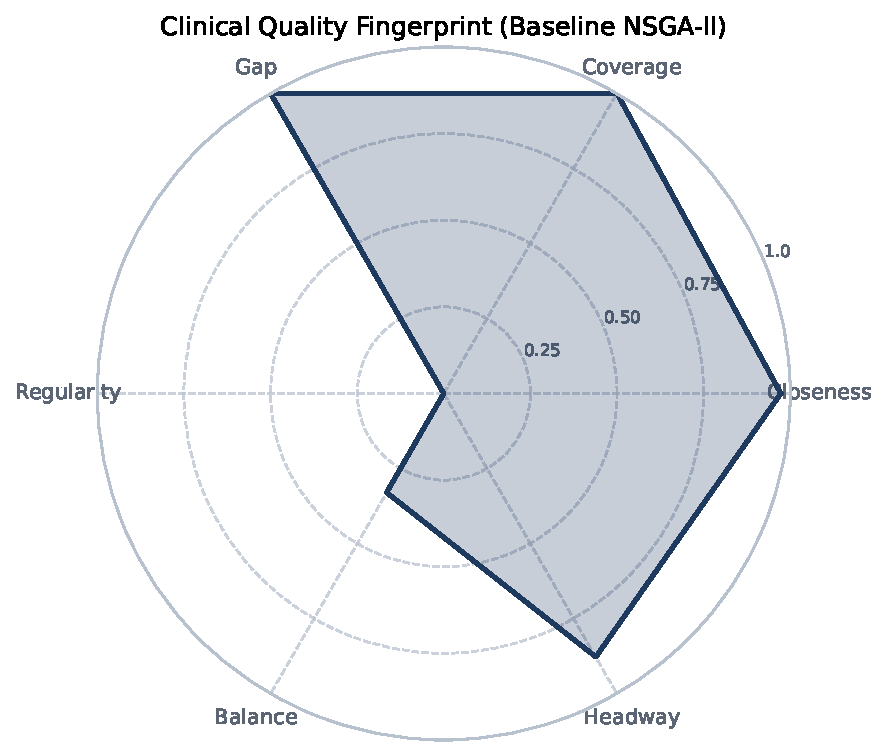
\includegraphics[width=\linewidth,height=.56\textheight,keepaspectratio]{figures/example_14_01_radar.pdf}
\end{column}
\end{columns}
\vspace{.01cm}\textbf{Contraste:} boa proximidade e cobertura não garantem espaçamentos regulares.
\end{frame}

\begin{frame}[fragile]{Exemplo FAIR 14 — ECDF: onde estão as caudas de erro?}
\begin{lstlisting}[style=python,basicstyle=\ttfamily\fontsize{7.5}{9}\selectfont]
mb.view.ecdf(exp1, ground_truth=gt, metric='closeness')
mb.view.ecdf(exp1, ground_truth=gt, metric='coverage')
\end{lstlisting}
\begin{columns}[T,onlytextwidth]
\begin{column}{.49\textwidth}\centering
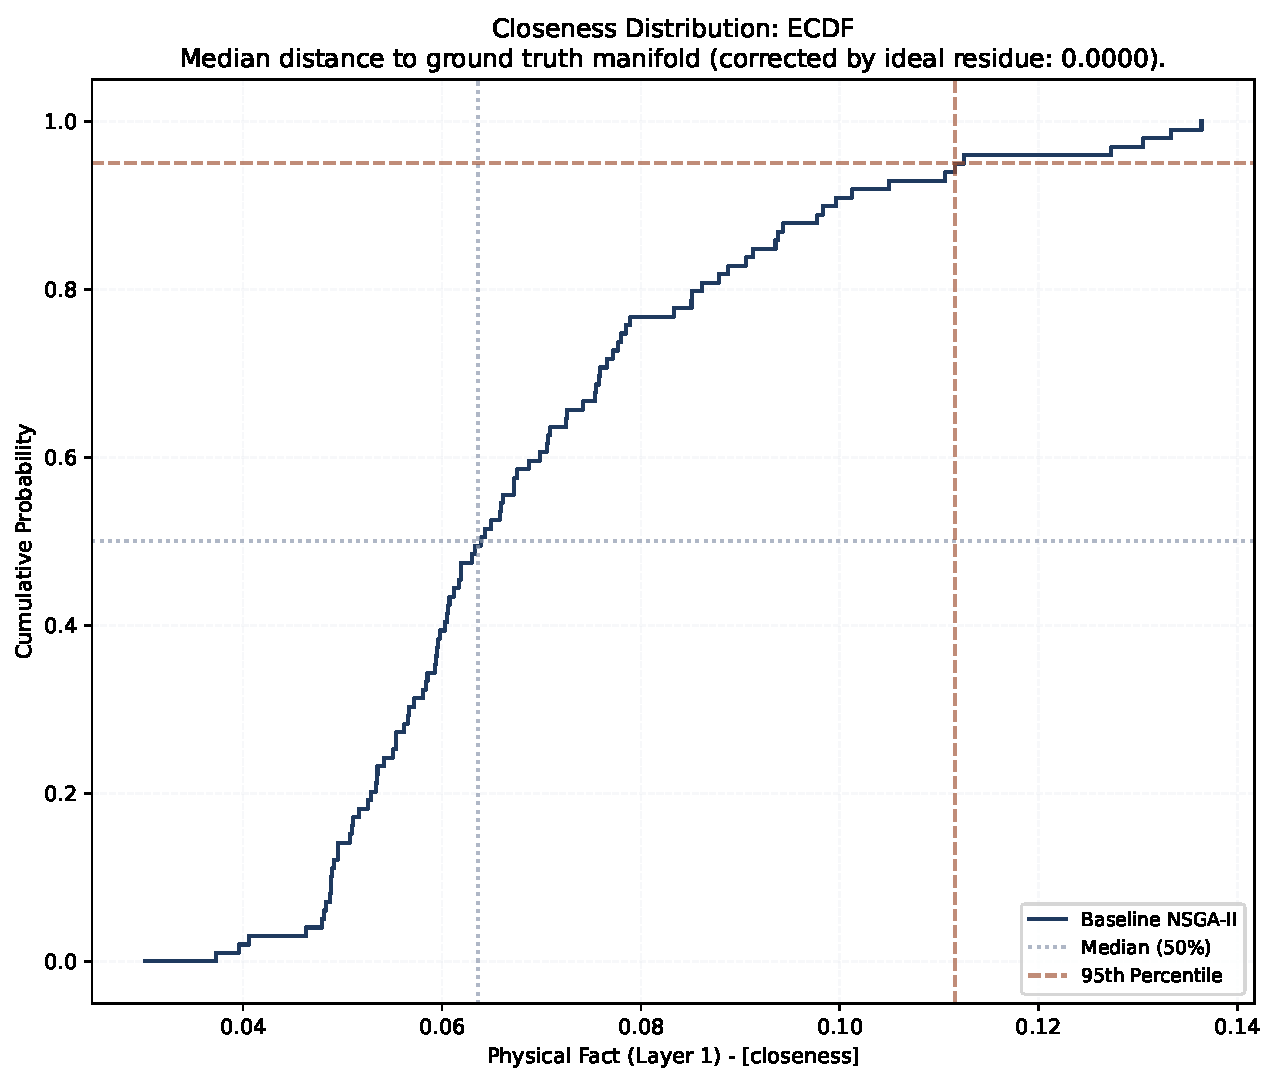
\includegraphics[width=\linewidth,height=.45\textheight,keepaspectratio]{figures/example_14_02_ecdf.pdf}
\par\scriptsize Closeness: distâncias $P\to R$.
\end{column}
\begin{column}{.49\textwidth}\centering
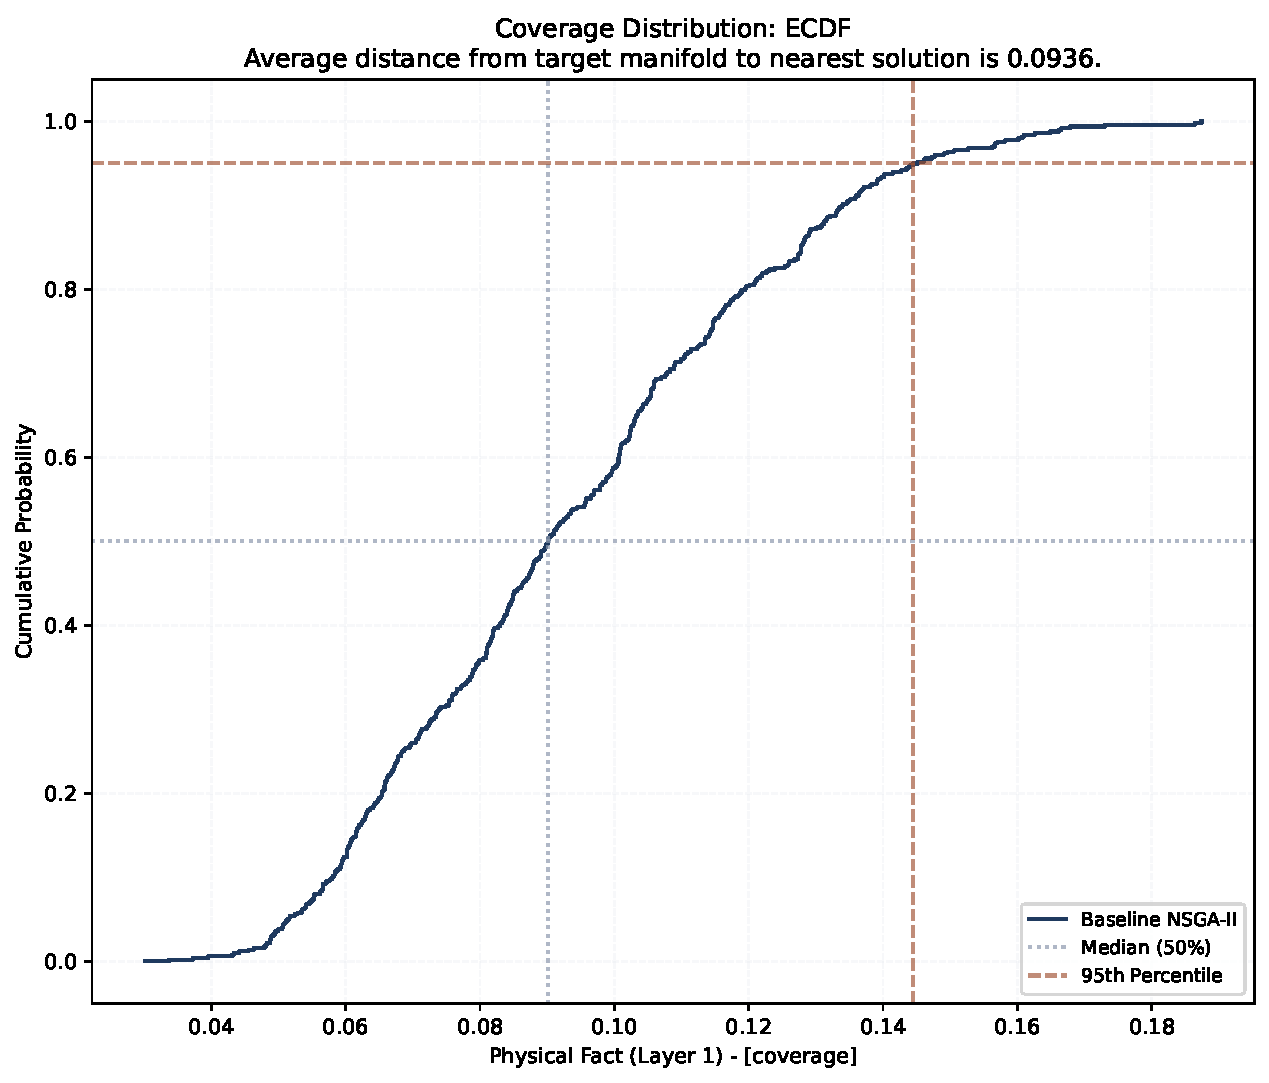
\includegraphics[width=\linewidth,height=.45\textheight,keepaspectratio]{figures/example_14_03_ecdf.pdf}
\par\scriptsize Coverage: distâncias $R\to P$.
\end{column}
\end{columns}
\vspace{.02cm}\textbf{Como ler:} para cada distância no eixo horizontal, a curva indica a fração de observações com erro até aquele limiar. A curva de coverage estende-se mais à direita, revelando regiões do GT relativamente mais distantes das soluções.
\end{frame}

\begin{frame}[fragile]{Exemplo FAIR 14 — Histogramas: concentração e dispersão dos erros}
\begin{lstlisting}[style=python,basicstyle=\ttfamily\fontsize{7.4}{9}\selectfont]
mb.view.density(exp1, domain='clinic', ground_truth=gt, metric='closeness')
mb.view.density(exp1, domain='clinic', ground_truth=gt, metric='coverage')
\end{lstlisting}
\begin{columns}[T,onlytextwidth]
\begin{column}{.49\textwidth}\centering
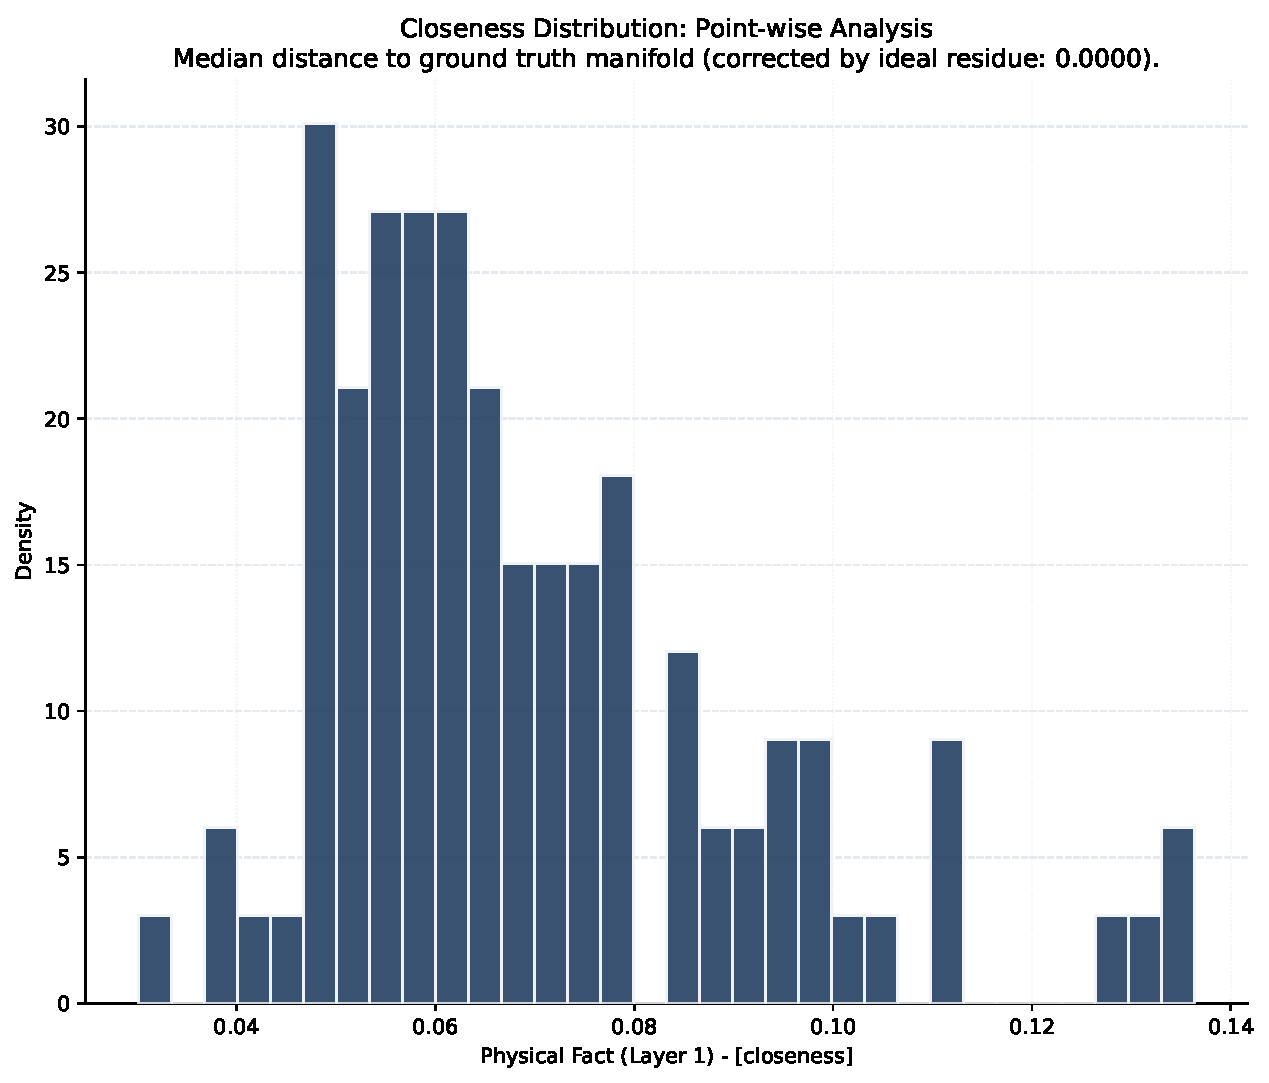
\includegraphics[width=\linewidth,height=.34\textheight,keepaspectratio]{figures/example_14_04_density.pdf}
\par\scriptsize Closeness: erros por solução obtida.
\end{column}
\begin{column}{.49\textwidth}\centering
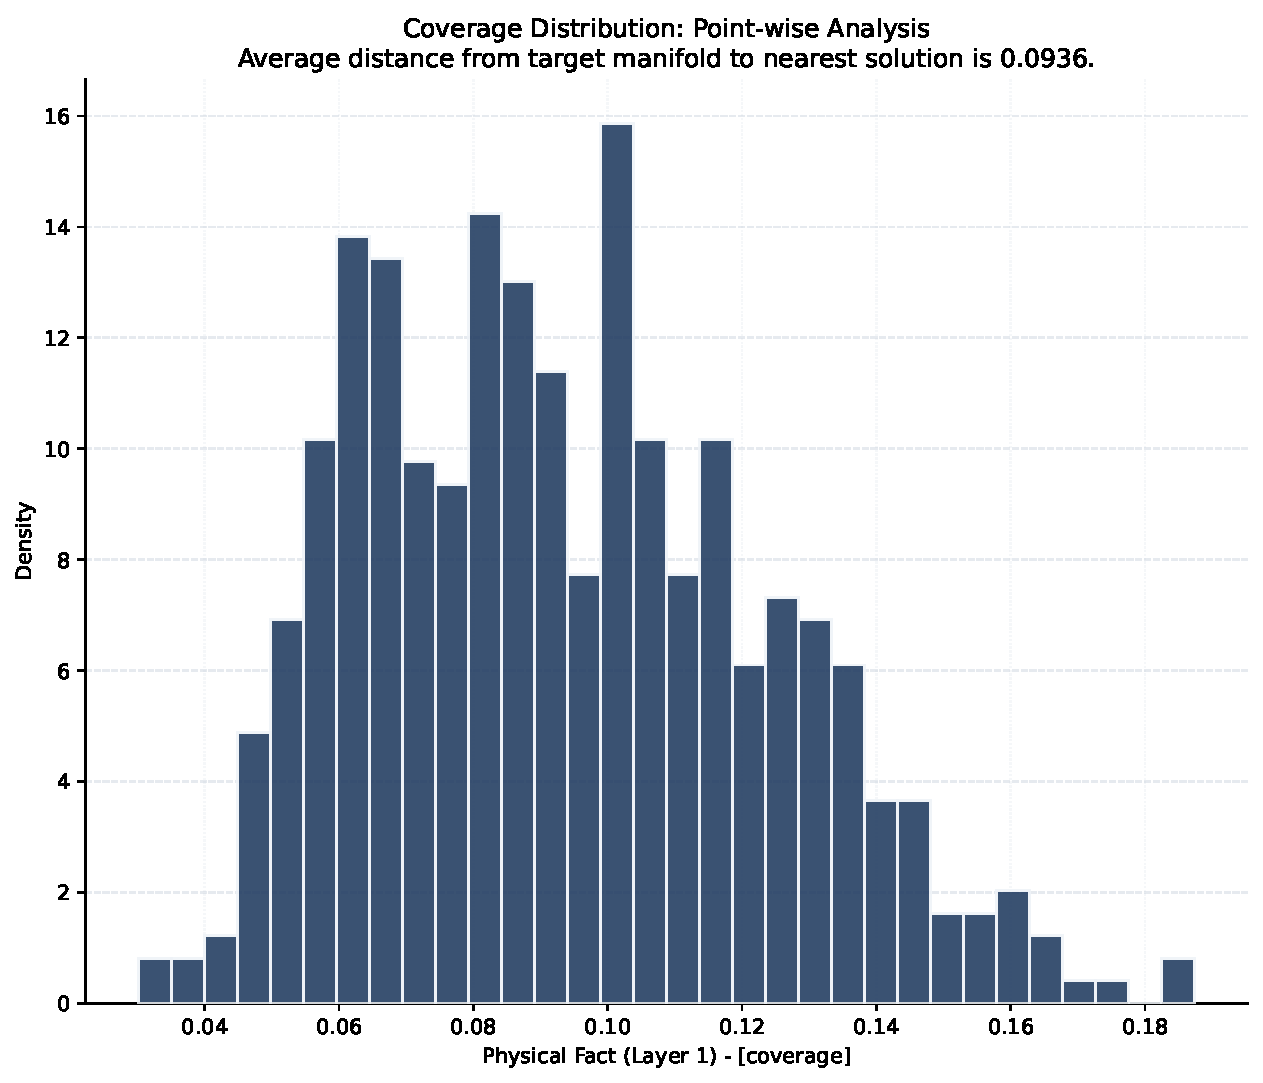
\includegraphics[width=\linewidth,height=.34\textheight,keepaspectratio]{figures/example_14_05_density.pdf}
\par\scriptsize Coverage: erros por ponto de referência.
\end{column}
\end{columns}
\vspace{.01cm}\textbf{Leitura:} closeness concentra erros pequenos; coverage apresenta distribuição mais larga e cauda direita. Algumas regiões do GT estão mais afastadas da população. Alturas brutas não são comparáveis entre amostras de tamanhos distintos.
\end{frame}

\begin{frame}[fragile]{Exemplo FAIR 14 — Históricos: quando ocorreu a melhora?}
\begin{lstlisting}[style=python,basicstyle=\ttfamily\fontsize{7.4}{9}\selectfont]
mb.view.history(exp1, domain='clinic', ground_truth=gt, metric='closeness')
mb.view.history(exp1, domain='clinic', ground_truth=gt, metric='coverage')
\end{lstlisting}
\begin{columns}[T,onlytextwidth]
\begin{column}{.49\textwidth}\centering
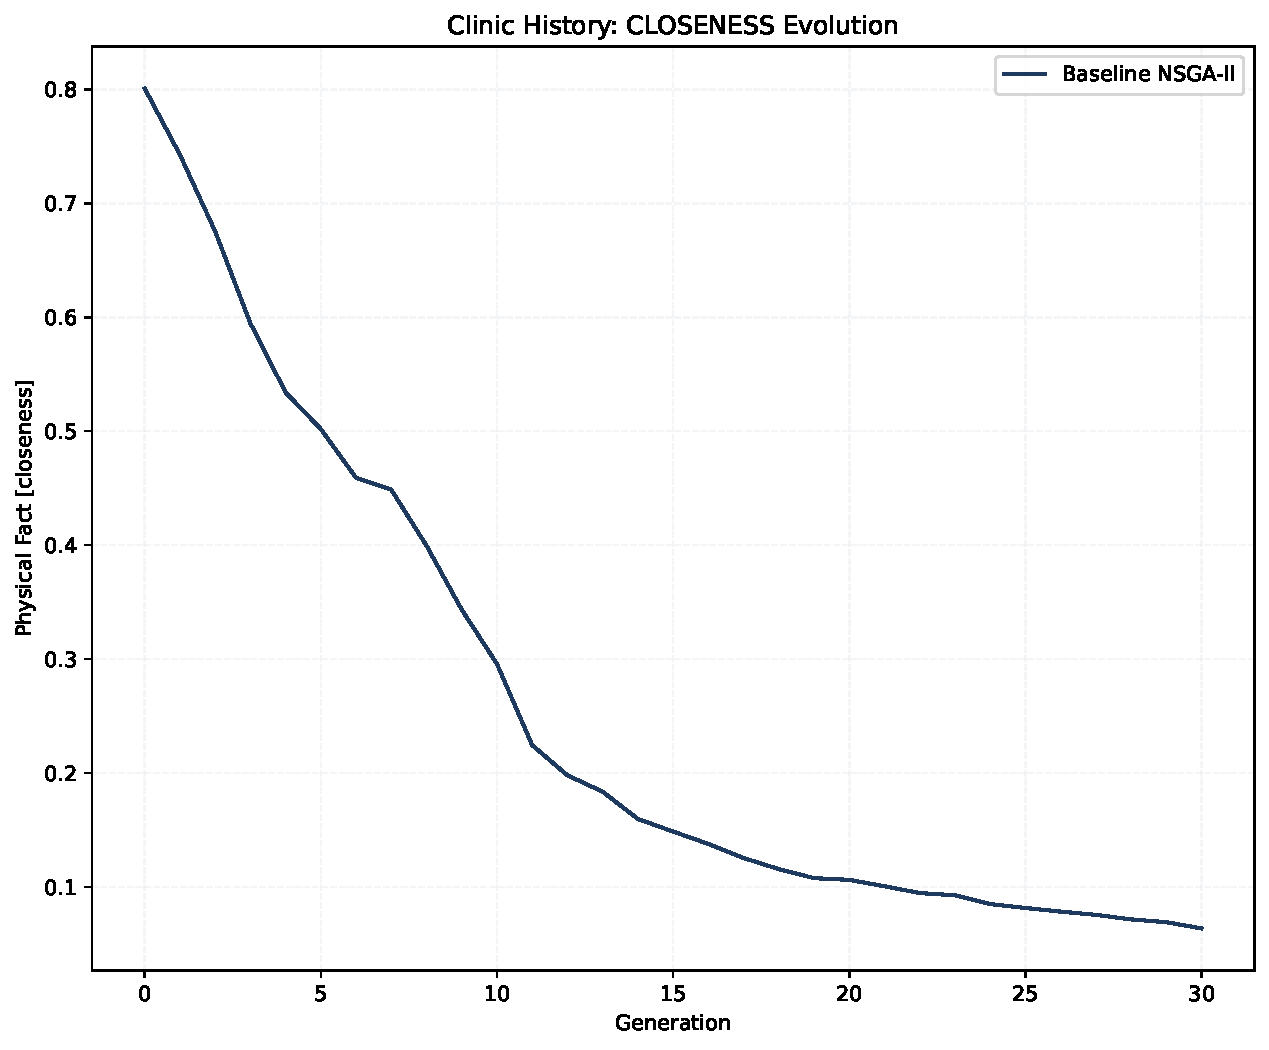
\includegraphics[width=\linewidth,height=.44\textheight,keepaspectratio]{figures/example_14_06_history.pdf}
\par\scriptsize Erro físico de closeness por geração.
\end{column}
\begin{column}{.49\textwidth}\centering
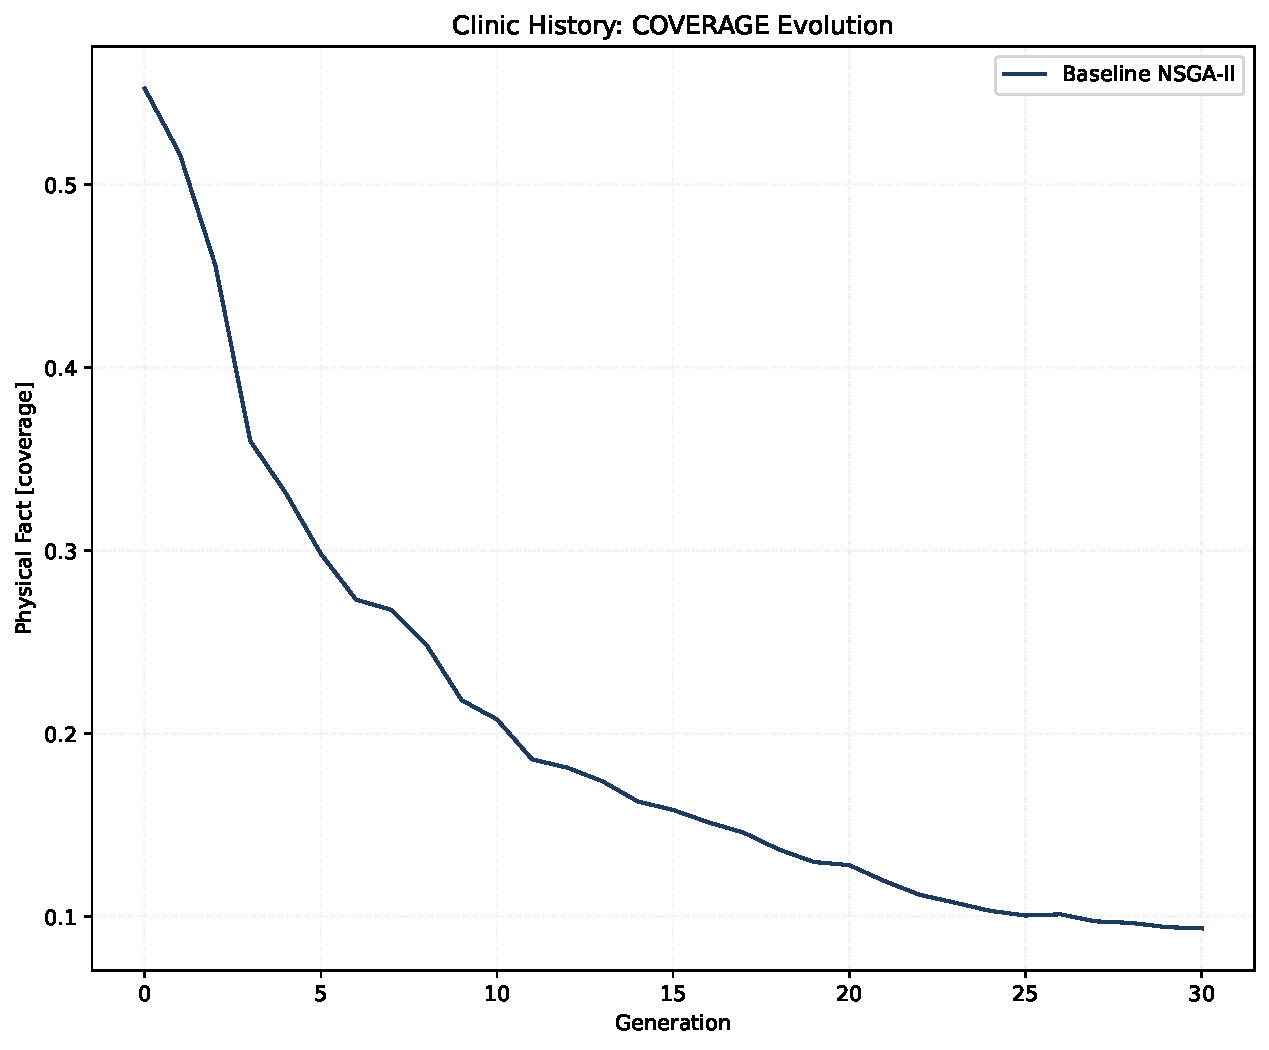
\includegraphics[width=\linewidth,height=.44\textheight,keepaspectratio]{figures/example_14_07_history.pdf}
\par\scriptsize Erro físico de coverage por geração.
\end{column}
\end{columns}
\vspace{.03cm}\textbf{Interpretação:} ambas as medidas caem ao longo da execução, sobretudo nas gerações iniciais; a cobertura final ainda é menos favorável que a proximidade. O radar resume o estado final, mas não mostra essa trajetória.
\end{frame}

\begin{frame}[fragile]{Exemplo FAIR 18 — Calibrar um novo problema e tamanho}
\textbf{DTLZ2 com 4 objetivos; NSGA-III, 40 indivíduos, 20 gerações.}\par\smallskip
\begin{lstlisting}[style=python,basicstyle=\ttfamily\fontsize{8.0}{10}\selectfont]
mop = mb.mops.DTLZ2(M=4)
exp = mb.experiment(
    mop=mop, moea=mb.moeas.NSGA3(population=40, generations=20))
exp.run(repeat=1)
mop.calibrate(size=40, source_baseline='dtlz2_m4_demo.json',
              force=True)
resultado = mb.clinic.audit(
    exp, source_baseline='dtlz2_m4_demo.json')
resultado.report()
\end{lstlisting}
\vspace{.05cm}\textbf{Resultado:} os 40 indivíduos finais são não dominados. A auditoria descreve convergência favorável e fragilidades em cobertura, continuidade e regularidade.
\par\smallskip\textbf{Importante:} este exemplo está na \textbf{seção 6.0.6.5} (Código 6.6) da monografia. \emph{Não} corresponde aos quadros do apêndice.
\end{frame}

\begin{frame}{Exemplo FAIR 18 — O que o arquivo auxiliar preserva?}
\textbf{Uma régua clínica requer o problema e a cardinalidade para os quais foi calibrada.}\par\medskip
\begin{center}
\begin{tikzpicture}[node distance=2.2cm, every node/.style={align=center,font=\small}]
\node[draw=navy,rounded corners,minimum width=2.7cm,minimum height=1.15cm] (m) {DTLZ2 ($M=4$)\\$K=40$};
\node[draw=navy,rounded corners,right=of m,minimum width=3cm,minimum height=1.15cm] (c) {\texttt{mop.calibrate()}\\referência e baselines};
\node[draw=navy,rounded corners,right=of c,minimum width=2.7cm,minimum height=1.15cm] (a) {\texttt{mb.clinic.audit()}\\Q-scores};
\draw[-{Stealth[length=2.6mm]},thick] (m)--(c);
\draw[-{Stealth[length=2.6mm]},thick] (c)--node[above,font=\scriptsize]{\texttt{.json} (sidecar)} (a);
\end{tikzpicture}
\end{center}
\vspace{.20cm}
\textbf{Por que isso importa?} O mesmo erro físico pode corresponder a um Q-score diferente quando mudam a geometria do MOP ou a resolução da aproximação. O arquivo \texttt{dtlz2\_m4\_demo.json} registra a calibração empregada, permitindo reutilizá-la na análise.
\par\medskip
\textbf{Limite do experimento:} 40 soluções não dominadas e boa proximidade não demonstram, por si, cobertura e distribuição adequadas na frente de quatro objetivos.
\end{frame}

\begin{frame}{Comparações adicionais — auditoria histórica do MoeaBench}
\textbf{Fonte independente:} \texttt{calibration/audit\_report.html}, gerado com MoeaBench \textbf{v0.14.0}. O relatório apresenta 30 execuções independentes e comparação de algoritmos em DTLZ e DPF.
\par\medskip
\begin{itemize}
\item Os resultados abaixo são \textbf{Q-scores reportados}, não projeções das execuções dos exemplos 11--18.
\item Cada problema possui sua própria calibração. Comparações quantitativas são mais apropriadas \textbf{dentro do mesmo MOP} e protocolo.
\item O relatório atribui \textbf{orçamentos de gerações distintos} a determinados algoritmos; logo, diferenças entre eles não devem ser interpretadas como evidência isolada de superioridade em orçamento igual.
\end{itemize}
\vspace{.20cm}
\textbf{Pergunta:} o que muda quando observamos separadamente as seis dimensões em vez de resumir o desempenho por HV, GD ou IGD?
\par\medskip
{\scriptsize Fonte: github.com/monacofj/moeabench/blob/main/calibration/audit\_report.html (v0.14.0).}
\end{frame}

\begin{frame}{Auditoria v0.14.0 — DTLZ2: proximidade similar, regularidade distinta}
\begin{columns}[T,onlytextwidth]
\begin{column}{.66\textwidth}\centering
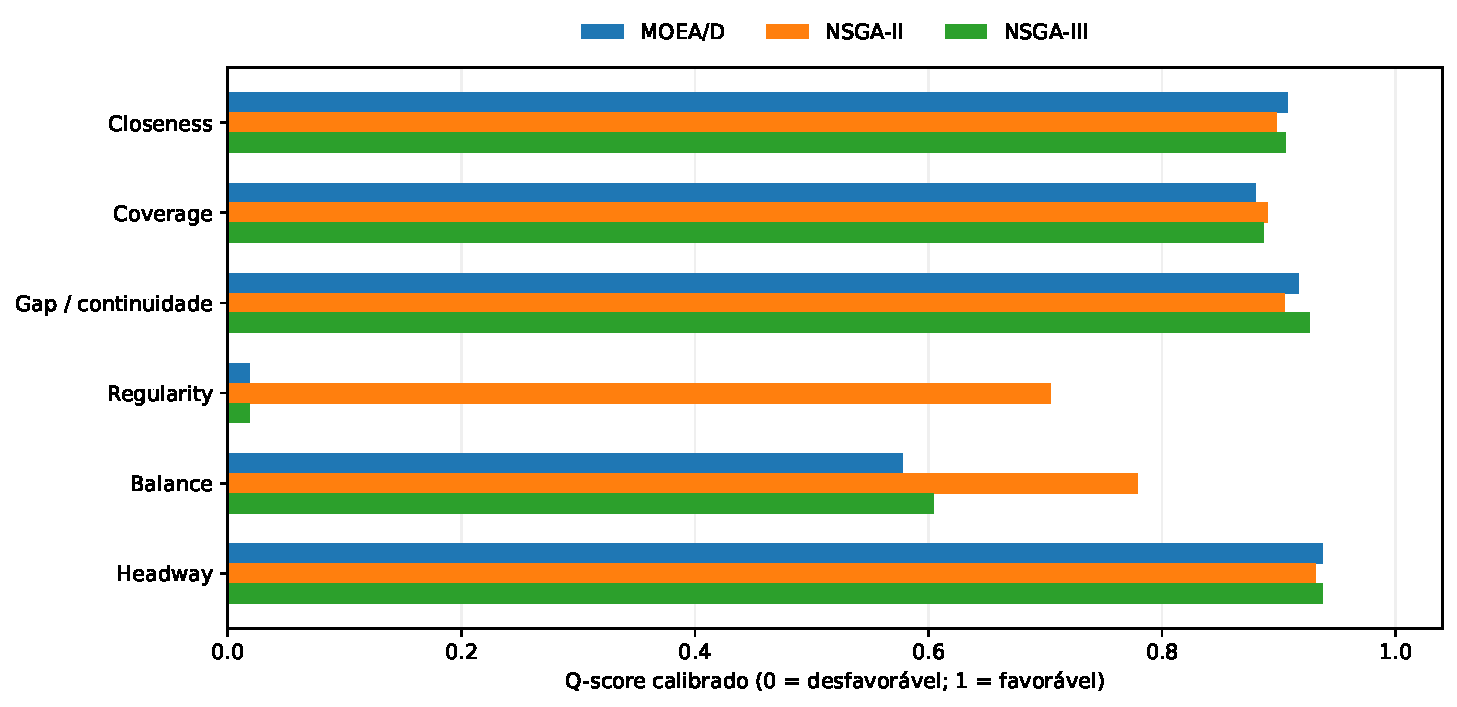
\includegraphics[width=\linewidth,height=.67\textheight,keepaspectratio]{figures/audit_dtlz2_qscores.pdf}
\end{column}
\begin{column}{.32\textwidth}
\textbf{Closeness}\par
MOEA/D: 0,907\par
NSGA-II: 0,898\par
NSGA-III: 0,906
\par\medskip
\textbf{Regularity}\par
MOEA/D: \textbf{0,019}\par
NSGA-II: \textbf{0,704}\par
NSGA-III: \textbf{0,019}
\end{column}
\end{columns}
\vspace{.04cm}\textbf{Interpretação:} todos se aproximaram do GT, mas a distribuição dos espaçamentos locais é muito mais favorável no resultado do NSGA-II. A avaliação de \emph{closeness} isolada esconderia esse contraste.
\par{\scriptsize Dados do relatório v0.14.0, DTLZ2 ($M=3$); configurações e gerações não são idênticas.}
\end{frame}

\begin{frame}{Auditoria v0.14.0 — DPF1: convergência não basta}
\begin{columns}[T,onlytextwidth]
\begin{column}{.66\textwidth}\centering
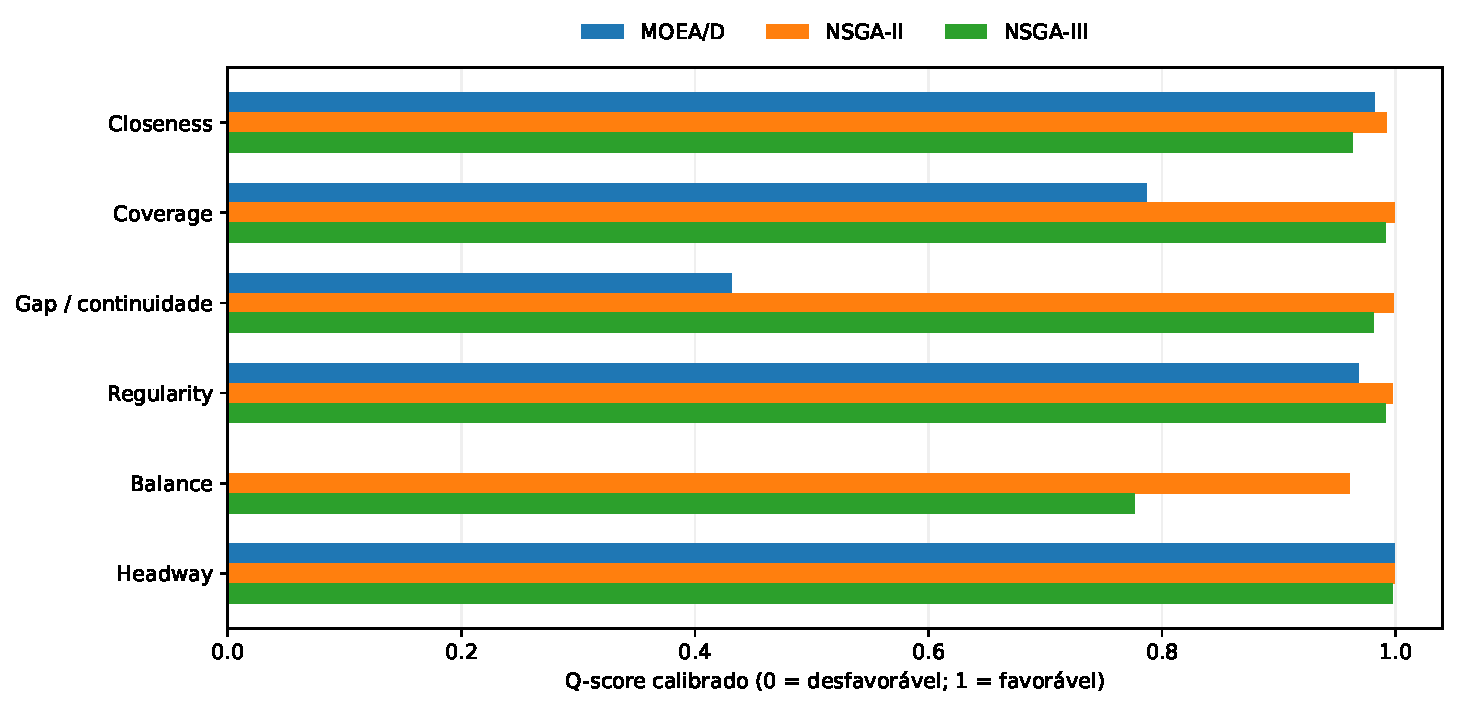
\includegraphics[width=\linewidth,height=.67\textheight,keepaspectratio]{figures/audit_dpf1_qscores.pdf}
\end{column}
\begin{column}{.32\textwidth}
\textbf{MOEA/D:}\par
Closeness \textbf{0,982}\par
Headway \textbf{0,999}\par
Gap/continuidade \textbf{0,431}\par
Balance \textbf{0,000}
\par\medskip
\textbf{NSGA-II:}\par
Gap/continuidade 0,998\par
Balance 0,960
\end{column}
\end{columns}
\vspace{.04cm}\textbf{Interpretação:} o MOEA/D apresenta convergência favorável, mas forte desequilíbrio regional e problemas de continuidade. O NSGA-II recebeu avaliações mais favoráveis para essas propriedades \emph{neste protocolo específico}.
\par{\scriptsize Relatório v0.14.0, DPF1 ($M=3$). ``Continuidade'' é o nome adotado no relatório para a dimensão relacionada a gap. Orçamentos de gerações distintos.}
\end{frame}

\begin{frame}{Auditoria v0.14.0 — DTLZ1: concordância em convergência, divergência estrutural}
\begin{columns}[T,onlytextwidth]
\begin{column}{.66\textwidth}\centering
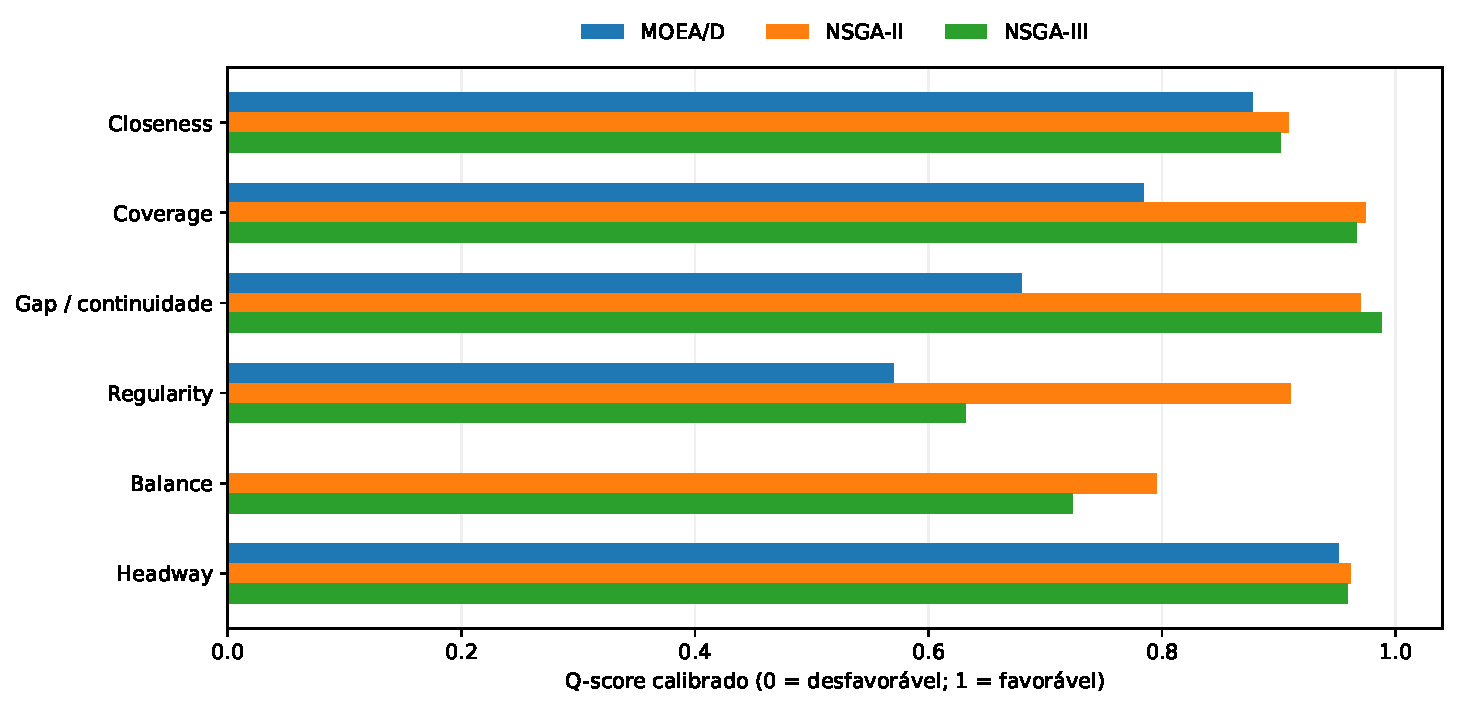
\includegraphics[width=\linewidth,height=.66\textheight,keepaspectratio]{figures/audit_dtlz1_qscores.pdf}
\end{column}
\begin{column}{.32\textwidth}
\textbf{Balance}\par
MOEA/D: \textbf{0,000}\par
NSGA-II: \textbf{0,795}\par
NSGA-III: \textbf{0,723}
\par\medskip
\textbf{Headway}\par
Todos: 0,951--0,961
\end{column}
\end{columns}
\vspace{.04cm}\textbf{Interpretação:} um progresso longitudinal semelhante convive com diferenças expressivas na ocupação regional. Headway responde \emph{quanto se progrediu}; balance, \emph{onde ficaram distribuídas as alternativas}.
\par{\scriptsize Dados do relatório v0.14.0, DTLZ1 ($M=3$); não confundir com a execução isolada do exemplo 13.}
\end{frame}

\begin{frame}{O que as análises clínicas acrescentaram aos experimentos?}
\begin{columns}[T,onlytextwidth]
\begin{column}{.49\textwidth}
\textbf{Exemplo 11 (DPF)}\par
Muitas soluções não dominadas não asseguram proximidade ao GT.
\par\medskip
\textbf{Exemplo 13 (DTLZ1)}\par
Closeness e headway altos podem coexistir com cobertura e estrutura espacial deficientes.
\par\medskip
\textbf{Exemplo 14 (DTLZ2)}\par
ECDFs, histogramas e históricos explicam as distâncias que deram origem ao radar.
\end{column}
\begin{column}{.49\textwidth}
\textbf{Auditoria histórica DTLZ2}\par
Closeness quase igual entre algoritmos, mas regularity bem diferente.
\par\medskip
\textbf{Auditoria histórica DPF1}\par
Convergência favorável pode coexistir com lacunas e forte desequilíbrio.
\par\medskip
\textbf{Exemplo 18 (4 objetivos)}\par
Q-scores dependem de calibração explícita da geometria e da cardinalidade.
\end{column}
\end{columns}
\vspace{.14cm}
\textbf{Síntese:} FAIR oferece um diagnóstico multidimensional \emph{da frente resultante}, não uma declaração única de superioridade algorítmica. Cada comparação deve respeitar seu MOP, referência e orçamento experimental.
\end{frame}